\chapter{Resultados}
\label{section:Resultados}

Los resultados obtenidos después de haber realizado la parte técnica del proyecto son los siguientes:
\begin{itemize}
    \item Hemos inspeccionado exhaustivamente el estado del arte en entornos multiagente y plataformas open source que pudieran servir como posibles entornos multiagente. Más adelante conseguimos definir unas métricas cualitativas para evaluar los entornos que habíamos encontrado.
    \item Hemos desarrollado un entorno con capacidad de entrenar a 4 agentes como máximo. Este entorno obliga a la cooperación entre agentes y está basado en el juego open source \textit{Mari0}. El \textbf{input} de este entorno son las posibles acciones que puede realizar un jugador en este videojuego. El \textbf{output} es una imagen en formato RGB de dimensiones 600 x 800. Adicionalmente, hemos generado la documentación necesaria para que otros investigadores puedan usar el entorno para entrenar agentes. Aparte, hemos conseguido que nuestro entorno siguiera la estructura de creación de entornos de \textit{PettingZoo}. Este entorno disponible únicamente en el sistema operativo de Linux.
    \item Hemos conseguido además implementar la funcionalidad de que pueda jugar un humano y varias inteligencias artificiales a la vez, pero siempre con la restricción de 4 jugadores como máximo.
    \item Finalmente hemos entrenado un par de agentes usando PPO y CNN. Aun habiendo entrenado a estos agentes con 500000 iteraciones, desafortunadamente estos agentes no son capaces de resolver ni siquiera la primera parte del primer nivel de forma consistente. Creemos que esto se debe a que el entorno es realmente complicado. Los agentes deben aprender las mecánicas del juego y aun sin obtener ninguna recompensa aparente, solucionar el puzzle con una estrategia a largo plazo.

\end{itemize}

Finalmente tenemos motivos para pensar que la política de recompensas no es muy orientativa en el entorno. Como hemos explicado en previos apartados, el agente utiliza las recompensas para guiarse de optimalidad de sus acciones. En la Figura \ref {fig:cum} podemos observar la gráfica de las recompensas acumuladas del entorno durante el entrenamiento. La gráfica está acotada hasta las primeras 3000 acciones, ya que a partir de este momento se vuelve monótona. Podemos observar que durante las primeras 500 iteraciones existen varios picos. Podemos asociar estos picos al avance que realizan los agentes hacia el borde derecho del cuadrilátero. A partir de ese punto, la tendencia de la gráfica es monótona, ya que los agentes no son capaces de avanzar de este punto y solo obtienen una recompensa negativa por realizar una acción. Gracias a esta gráfica queda claro que los agentes no son capaces de resolver el primer problema.
\begin{figure}[ht]
    \centering
    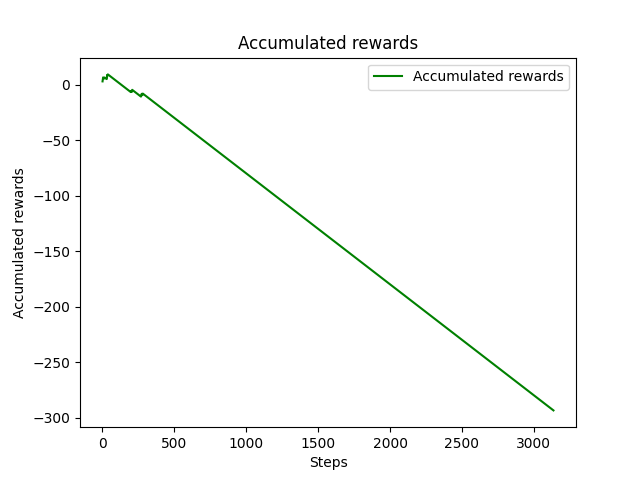
\includegraphics[width=0.9\textwidth]{img/rewards_cum.png}
    \caption{Recompensas acumuladas [Elaboración Propia]}
    \label{fig:cum}
\end{figure}


Sin embargo, observando las siguientes gráficas podemos concluir que el algoritmo considera que la política que ha implementado es óptima. En la Figura \ref{fig:kl} podemos observar la función de \textit{Kullback-Leibler divergence} aproximada. Se trata de la función aproximada, ya que calcular esta función directamente es computacionalmente muy costoso. Esta función sirve para comparar como una función de probabilidad se diferencia de otra. En nuestro caso se utiliza para medir la diferencia entre las políticas que utilizan nuestros agentes. La forma intuitiva de leer la gráfica es que a menor es el valor, menos varían las políticas. Por norma general, cuando un agente está aprendiendo a resolver un entorno, esta función comienza con valores altos y decrece hasta converger. Esto se debe a que a medida que el agente aprende, no es necesario que aplique cambios radicales a su política. Y esto es precisamente el comportamiento que podemos ver en nuestros agentes. Aparentemente el algoritmo considera que está solucionando el entorno. Esta gráfica también está acotada, ya que la tendencia es la misma a partir de las 50000 iteraciones.
\begin{figure}[ht]
    \centering
    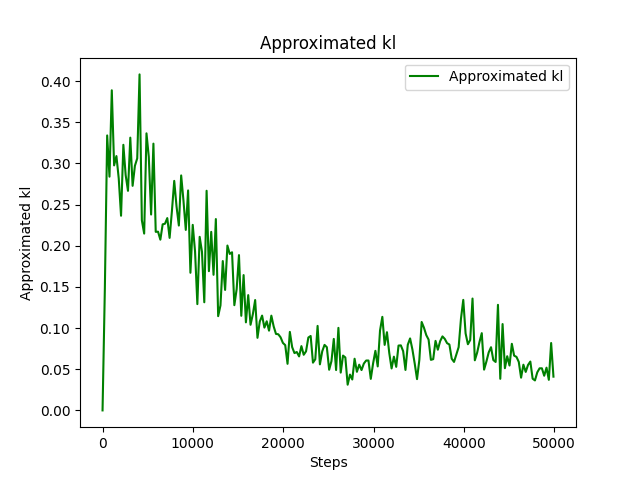
\includegraphics[width=0.9\textwidth]{img/approx_kl.png}
    \caption{Función de \textit{Kullback-Leibler divergence} aproximada [Elaboración Propia]}
    \label{fig:kl}
\end{figure}

La Figura \ref{fig:loss} corrobora estas conclusiones. Esta gráfica representa la diferencia de entre el valor esperado de un estado concreto y el valor empírico de este estado. Cuando hablamos del valor de un estado podemos pensar que se trata básicamente de las recompensas que se esperan obtener comenzando a partir de este estado. Esto incluye las recompensas inmediatas recibidas en este estado además de las futuras posibles recompensas. Por norma general, cuando el valor de esta función es cercano a 0 significa que el algoritmo de aprendizaje es capaz de predecir las posibles recompensas de un cierto estado y por lo tanto está aprendiendo correctamente como solucionar el entorno. En nuestro caso, podemos observar que se trata de este caso. Los picos que podemos ver en la figura constituyen algunas recompensas inesperadas, pero no son nada habituales en nuestra función por lo que no es necesario darles mucha importancia.
\begin{figure}[ht]
    \centering
    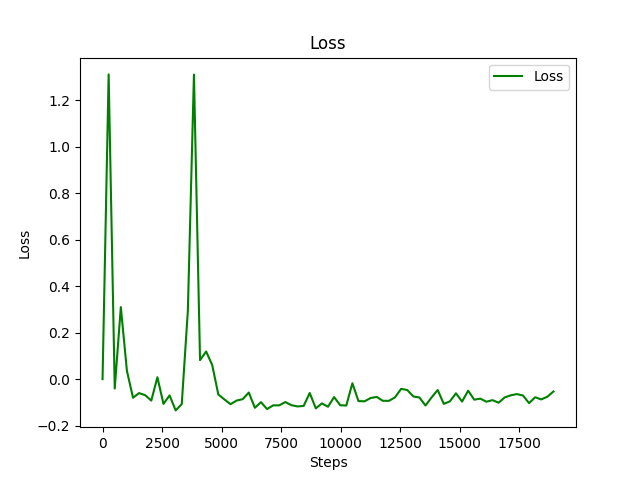
\includegraphics[width=0.9\textwidth]{img/loss.png}
    \caption{Función de perdida [Elaboración Propia]}
    \label{fig:loss}
\end{figure}

Gracias a las dos gráficas anteriores podemos concluir que el algoritmo considera que está solucionando el entorno, mientras que la Figura \ref{fig:cum} nos confirma que esto no así. Si esto sucede, suele implicar que la política de recompensas que guía al algoritmo no es muy adecuada y no lo está guiando efectivamente. Ya que desarrollar un sistema de recompensas no era el objetivo de este TFG, sino crear un modelo de referencia, encontrar un sistema de recompensas más efectivo queda como trabajo futuro.



El código de este entorno se encuentra en \cite {repo}.
 

